\documentclass[a4paper,titlepage,12pt]{article}
\usepackage[utf8]{inputenc} %Make sure all UTF8 characters work in the document
\usepackage{color}
\usepackage{graphicx}
\usepackage{titling}
\usepackage{tabularx}
\usepackage{longtable}
\usepackage[yyyymmdd]{datetime}
\usepackage[figurename=Figur]{caption}
\usepackage{pbox}
\usepackage{booktabs}

%Set page size
\usepackage{geometry}
\geometry{margin=3cm}

\renewcommand{\dateseparator}{-}
\renewcommand{\contentsname}{Innehållsförteckning}

%%%%%%%%%%%%%%%%%%%%%%%%%%%%%%%
% Header and footer
%%%%%%%%%%%%%%%%%%%%%%%%%%%%%%%
\usepackage{fancyhdr}
\pagestyle{fancy}

\lhead{
\includegraphics[width=0.15\linewidth]{../images/logo_full.png}}
\chead{Projektplan för sexbent robot}
\rhead{\today}
\setlength\headheight{26pt} 

\lfoot{TSEA29 --- KMM \\ LIPS Projektplan}
\rfoot{Grupp 9 \\ LiTHe Hex}

\pretitle{%
    \begin{center}
        \LARGE
        
\includegraphics[width=6cm]{../images/logo_full.png}\\[\bigskipamount]
}

\posttitle{\end{center}}

\newcounter{milNr}
\setcounter{milNr}{0}
\newcommand{\nextMilNr}{\stepcounter{milNr}\arabic{milNr}}

\newcounter{bpNr}
\setcounter{bpNr}{-1}
\newcommand{\nextBPNr}{\stepcounter{bpNr}\arabic{bpNr}}

\newcounter{aktNr}
\setcounter{aktNr}{0}
\newcommand{\nextAktNr}{\stepcounter{aktNr}\arabic{aktNr}}

\begin{document}
    \title{\LARGE
        \textbf{Projektplan för sexbent robot} \\
        \vspace*{0.5\baselineskip}
        \large
        Redaktör Malcolm Vigren \\
        Grupp 9 \\
        \small
        \vspace*{0.5\baselineskip}
        Version 0.1}

    \date{\today}

	\maketitle
	
	\newpage
	
	\begin{center}

		%%%%%%%%%%%%%%%%%%%%%%%%%%%%%%%%%%%%%%%%%%%%%%%%%%%%%%%%%%%%%%%%%%%%%%%%%%%%%%%%%
		%						Medlemmar
		%%%%%%%%%%%%%%%%%%%%%%%%%%%%%%%%%%%%%%%%%%%%%%%%%%%%%%%%%%%%%%%%%%%%%%%%%%%%%%%%%

		\section*{Projektidentitet}
		Grupp 9, Ht 2016, LiTHe Hex

		Linköpings Tekniska Högskola, ISY

		\renewcommand*{\arraystretch}{1.4}
		\begin{longtable}[c]{ l l l }
			\textbf{Namn} & \textbf{Ansvar} & \textbf{E-post} \\ \midrule
			Emil Segerbäck & & emise935@student.liu.se \\ \midrule
			Frans Skarman & Dokumentansvarig & frask812@student.liu.se \\ \midrule
			Hannes Tuhkala & & hantu447@student.liu.se \\ \midrule
			Malcolm Vigren & Projektledare & malvi108@student.liu.se \\ \midrule
			Noak Ringman &  & noari093@student.liu.se \\ \midrule
			Olav Övrebö &  & olaov121@student.liu.se \\ \midrule
			Robin Sliwa &  & robsl733@student.liu.se \\
		\end{longtable}

		\centering
		\textbf{Kursansvarig}: Tomas Svensson Rum 3B:528 013--28 13 68 tomas.svensson@liu.se

		\newpage
		\tableofcontents
		\newpage


		%%%%%%%%%%%%%%%%%%%%%%%%%%%%%%%%%%%%%%%%%%%%%%%%%%%%%%%%%%%%%%%%%%%%%%%%%%%%%%%%%
		%						Historik
		%%%%%%%%%%%%%%%%%%%%%%%%%%%%%%%%%%%%%%%%%%%%%%%%%%%%%%%%%%%%%%%%%%%%%%%%%%%%%%%%%

		\section*{Dokumenthistorik}
		\renewcommand*{\arraystretch}{1.4}
		\begin{longtable}[c]{ l l l l l }
			\textbf{Version} & \textbf{Datum} & \textbf{Utförda förändringar} 
			& \textbf{Utförda av} & \textbf{Granskad} \\ \midrule

			0.1 & 2016--09--20 & Första utkastet & Projektgruppen & \\
		\end{longtable}
	\end{center}

	\newpage

	\section{Beställare}
	Beställare är Tomas Svensson, lektor vid Linköpings tekiska högskola. \\
  Kontaktdata: Rum 3B:528 013–28 13 68 tomas.svensson@liu.se

	%%%%%%%%%%%%%%%%%%%%%%%%%%%%%%%%%%%%%%%%%%%%%%%%%%%%%%%%%%%%%%%%%%%%%%%%%%%%%%%%%
	%						Översikt
	%%%%%%%%%%%%%%%%%%%%%%%%%%%%%%%%%%%%%%%%%%%%%%%%%%%%%%%%%%%%%%%%%%%%%%%%%%%%%%%%%

	\newpage
	\section{Översiktlig beskrivning av projektet}
	Text

	\subsection{Syfte och mål}
	Syftet och målet med projektet är att utveckla en sexbent robot som själv
    kan navigera sig ut ur en labyrint. I labyrinten bör roboten även kunna ta
    sig över hinder för att komma vidare.

    % TODO varför ska vi lägga till "specifika syften som berör projektet och
    % dess medlemmar"???!!??!
	
	
	\subsection{Leveranser}
	De dokument som ska levereras till kunden är: projektplan, tidplan,
    systemskiss, designspecifikation, teknisk dokumentation och
    användarhandledning. Slutleveransen består av en presentation av projektet,
    demonstration av roboten i autonomnt och manuellt läge i form av en tävling,
    samt överlämning av kod, hårdvara och dokumentation.
	
	
	\subsection{Begränsningar}
	Roboten behöver inte klara mer avancerade former på labyrinten än de som
    beskrivs i Bilaga A:\ Ban- och regelspecifikation.
	
	
	\section{Fasplan}
	Här var det text här var det text här var det text
	här var det text här var det text här var det text
	här var det text här var det text här var det text.
	
	% \subsection{Före projektstart}
    % Före projektstarten har en grupp bildats med 7 medlemmar, där varje medlem
    % har tilldelats ett eller flera ansvarsområden inom projektet. En
    % kravspecifikation har skrivits enligt projektdirektivet och godkänts av
    % beställaren. En projektplan, tidsplan och systemskiss har skrivits och
    % godkänts av beställaren.
	
	
	\subsection{Under projektet}
	Under projektet ska en designspecifikation skrivas med detaljerad
    information om hur roboten ska implementeras. I samband med slutskedet

	
	\subsection{Efter projektet}
    Projektet avslutas med slutleverans samt en efterstudie.
	
	
	\section{Organisationsplan för hela projektet}
    I detta avsnitt beskrivs hur projektet ska organiseras.

	\subsection{Organisationsplan per fas}
	\begin{center}
		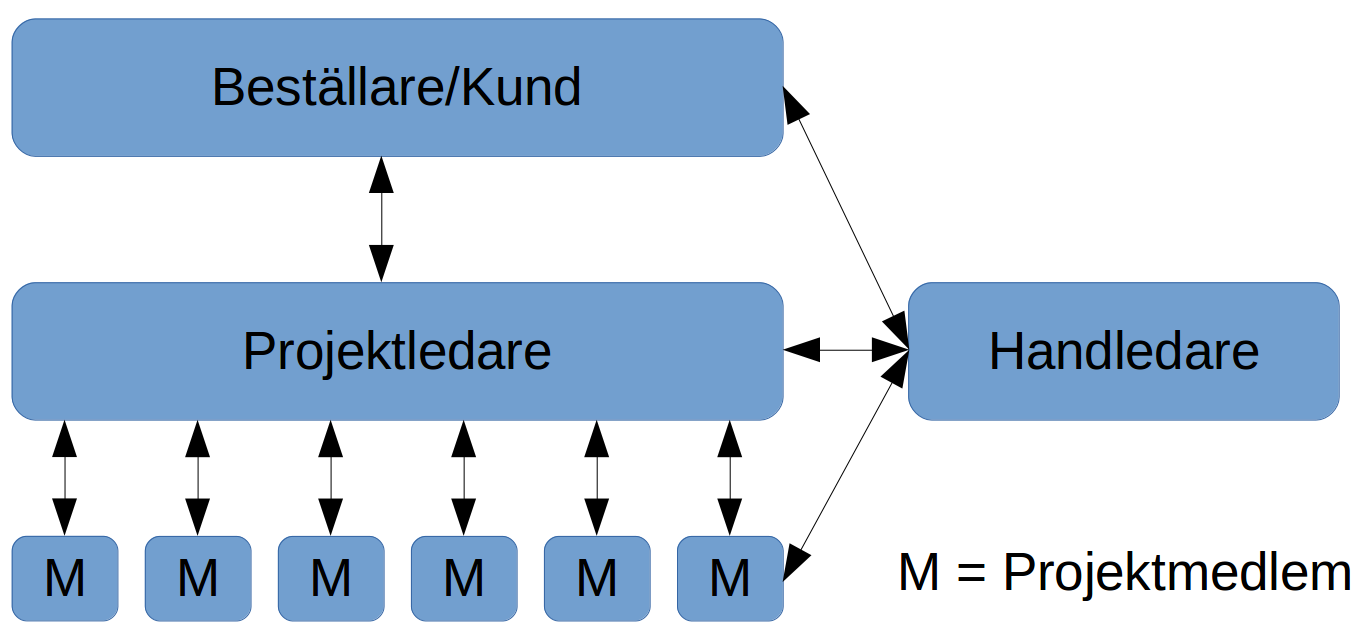
\includegraphics[width=0.8\linewidth]{images/projectroles.png}
	\end{center}
	Projektrollerna som ingår i detta projekt är: beställare/kund, handlerare,
	projektledare och projektmedlemmar. I beställarens arbetsuppgifter ingår saker
	som att fatta beslut om fortsättning av projektet vid beslutspunkter, godkänna
	ändringar under projektets gång, läsa statusrapporter och godkännande av
	projektets avslut. Arbetsuppgifterna för projektledaren är till stor del som
	de övriga projektmedlemmarna men det ingår även saker som att fördela
	arbetsuppgifter, planera och leda projektarbetet, se till att projektets mål
	nås och motivera projektmedlemmarna.
	% TODO: Finish this section
	
	% \subsection{Organisationsplan hos kunden}
	% Här var det text här var det text här var det text
	% här var det text här var det text här var det text
	% här var det text här var det text här var det text.
	% 
	 
	\subsection{Villkor för samarbetet inom projektgruppen}
	Här var det text här var det text här var det text
	här var det text här var det text här var det text
	här var det text här var det text här var det text.
	
	\subsection{Definition av arbetsinnehåll och ansvar}
	\begin{longtable}[c]{ c l>{\raggedright}p{0.6\textwidth} l l}
		\textbf{Nr} & \textbf{Förändring} & \textbf{Kravtext} & \textbf{Prioritet} 
			\\ \midrule

	\end{longtable}
	
	
	\section{Dokumentplan}
    Dokumenten lagras på GitHub och Git används för versionshantering av
    dokumenten, som skrivs i LaTeX. Alla projektmedlemmar har tillgång till
    samtliga dokument. All dokumentation, förutom kommentarer och doc-strängar
    i kod, är skriven på svenska.

    Stora ändringar ger inkrementering av heltalssiffran i versionsnumrena,
    medan små ändringar ger inkrementation av decimalsiffran.
	
    % FIXME kontrollera ansvarig och sånt
    % TODO lägg till eventuella fler interna dokument
    \begin{longtable}[c]{ l l l>{\raggedright}p{0.6\textwidth} l }
        \textbf{Dokument} & \textbf{Ansvarig/godkänns av} & \textbf{Syfte} & \textbf{Distribueras till} & \textbf{Färdigdatum} \\ \midrule
        
        Kravspecifikation & Beställare & Definierar alla krav på
        systemet & Beställare & 2016--09--13 \\ \midrule

        Projektplan & Beställare & <SOMETHING> & Beställare &
        2016--09--29 \\ \midrule

        Tidplan & Beställare & Planering för hur arbetstid ska
        fördelas. & Beställare & 2016--09--29  \\ \midrule
        
        Systemskiss & Beställare & Grov skiss och idéer för 
        implementation av systemet & Beställare & 2016--09--29 \\ \midrule

        Designspecifikation & Handledare & Detaljerad beskrivning av
        implementationen av systemet. & Handledare & 2016--11--04 \\ \midrule

        Tidrapporter & Beställare & Rapportering av använd arbetstid &
        Beställare & nån gång %TODO WHEN???
        \\ \midrule

        Teknisk dokumentation & Beställare & Teknisk beskriving av
        implementationen av den färdiga produkten. & Beställare &
        2016--12--17 \\ \midrule

        Användarhandledning & Beställare & En manual för användning av
        produkten & Beställare & 2016--12--17 \\ \midrule

        Efterstudie & Beställare & Utvärdering av projektet &
        Beställare & 2016--12--22  \\ \midrule
    \end{longtable}
	
	
	\section{Utvecklingsmetodik}
	Här var det text här var det text här var det text
	här var det text här var det text här var det text
	här var det text här var det text här var det text.
	
	
	\section{Utbildningsplan}
	Här var det text här var det text här var det text
	här var det text här var det text här var det text
	här var det text här var det text här var det text.
	
	
	\subsection{Egen utbildning}
	Här var det text här var det text här var det text
	här var det text här var det text här var det text
	här var det text här var det text här var det text.
	
	
%	\subsection{Kundens utbildning}
%	Här var det text här var det text här var det text
%	här var det text här var det text här var det text
%	här var det text här var det text här var det text.
	
	
	\section{Rapporteringsplan}
	Här var det text här var det text här var det text
	här var det text här var det text här var det text
	här var det text här var det text här var det text.
	
	
	\section{Mötesplan}
	Här var det text här var det text här var det text
	här var det text här var det text här var det text
	här var det text här var det text här var det text.
	
	
	\section{Resursplan}
	Här var det text här var det text här var det text
	här var det text här var det text här var det text
	här var det text här var det text här var det text.
	
	
	\subsection{Personer}
	Här var det text här var det text här var det text
	här var det text här var det text här var det text
	här var det text här var det text här var det text.
	
	
	\subsection{Material}
	Här var det text här var det text här var det text
	här var det text här var det text här var det text
	här var det text här var det text här var det text.
	
	
	\subsection{Lokaler}
	Här var det text här var det text här var det text
	här var det text här var det text här var det text
	här var det text här var det text här var det text.
	
	
	\subsection{Ekonomi}
	Här var det text här var det text här var det text
	här var det text här var det text här var det text
	här var det text här var det text här var det text.
	
	
	\section{Milstolpar och beslutspunkter}
	Här var det text här var det text här var det text
	här var det text här var det text här var det text
	här var det text här var det text här var det text.
	
	
	\subsection{Milstolpar}
	\begin{longtable}[c]{ c l c}
		\textbf{Nr} & \textbf{Beskrivning} & \textbf{Datum} \\ \midrule
		\nextMilNr{} & Kravspecifikationen är klar & 2016--09--13 \\ \midrule
		\nextMilNr{} & Projektplan, systemskiss och tidsplan är klar & -- \\ \midrule
		\nextMilNr{} & Designspecifikation är klar & -- \\ \midrule
	\end{longtable}
	
	
	\subsection{Beslutspunkter}
	\renewcommand*{\arraystretch}{1.4}
	\begin{longtable}[c]{ c l c}
		\textbf{Nr} & \textbf{Beskrivning} & \textbf{Datum} \\ \midrule
		\nextBPNr{} & Godkännande av projektdirektiv, beslut att starta förstudie & 2016--09--02 \\ \midrule
		\nextBPNr{} & Godkännande av kravspecifikation, beslut att starta förberedelsefasen & 2016--09--13 \\ \midrule
		\nextBPNr{} & Godkännande av projektplanering, beslut att starta utförandefasen & 2016--09--29 \\ \midrule
		\nextBPNr{} & Godkännande av designspecifikation, beslut att fortsätta
        utförandefasen & -- \\ \midrule
		\nextBPNr{} & Används ej & -- \\ \midrule
		\nextBPNr{} & Godkännande av produktens funktionalitet, beslut att leverera & -- \\ \midrule
		\nextBPNr{} & Godkännande av leverans, beslut att upplösa projektgruppen & -- \\ \midrule
	\end{longtable}
	
	
	\section{Aktiviteter}
	\renewcommand*{\arraystretch}{1.4}
	\begin{longtable}[c]{ c p{3cm} p{6cm} p{3cm} p{2cm}}
		\textbf{Nr} & \textbf{Aktivitet} & \textbf{Beskrivning} & \textbf{Beroende av aktivitet nr} & \textbf{Beräknad tid tim} \\ \midrule
		\nextAktNr{} & Inverse Kinematics & -- & -- & -- \\ \midrule
		\nextAktNr{} & Servokontroll & -- & -- & -- \\ \midrule
		\nextAktNr{} & Gångstil & -- & -- & -- \\ \midrule
		\nextAktNr{} & Kommunikation & -- & -- & -- \\ \midrule
		\nextAktNr{} & Golvhöjdsdetektion & -- & -- & -- \\ \midrule
		\nextAktNr{} & Stötdetektion & -- & -- & -- \\ \midrule
		\nextAktNr{} & Hindergång & -- & -- & -- \\ \midrule
		\nextAktNr{} & Kommunikation med motorikenhet & -- & -- & -- \\ \midrule
		\nextAktNr{} & Detektera återvändsgränser & -- & -- & -- \\ \midrule
		\nextAktNr{} & Kommunikation med sensorenhet & -- & -- & -- \\ \midrule
		\nextAktNr{} & Kommunikation med GUI & -- & -- & -- \\ \midrule
		\nextAktNr{} & Följa korridor & -- & -- & -- \\ \midrule
		\nextAktNr{} & Hinderdetektion & -- & -- & -- \\ \midrule
		\nextAktNr{} & Hinderhantering & -- & -- & -- \\ \midrule
		\nextAktNr{} & Beslutsfattning & -- & -- & -- \\ \midrule
		\nextAktNr{} & GUI kommandotolkning & -- & -- & -- \\ \midrule
		\nextAktNr{} & Telemetri & -- & -- & -- \\ \midrule
		\nextAktNr{} & Styrning & -- & -- & -- \\ \midrule
		\nextAktNr{} & Webbserver & -- & -- & -- \\ \midrule
		\nextAktNr{} & Frontend & -- & -- & -- \\ \midrule
		\nextAktNr{} & Joystick control & -- & -- & -- \\ \midrule
		\nextAktNr{} & Debug log & -- & -- & -- \\ \midrule
		\nextAktNr{} & Läsning av IR-sensor & -- & -- & -- \\ \midrule
		\nextAktNr{} & Kommunikation med centralenhet & -- & -- & -- \\ \midrule
		\nextAktNr{} & Läsning av gyro-sensor & -- & -- & -- \\ \midrule
		\nextAktNr{} & Läsning av LIDAR & -- & -- & -- \\ \midrule
		\nextAktNr{} & Brusdetektion av IR-sensor & -- & -- & -- \\ \midrule
		\nextAktNr{} & Integral av gyro & -- & -- & -- \\ \midrule
		\nextAktNr{} & Multiplexning A/D omvandlare & -- & -- & -- \\ \midrule
		\nextAktNr{} & Enhetskonvertering & -- & -- & -- \\ \midrule
		\nextAktNr{} & Buffertid & -- & -- & -- \\ \midrule
		\nextAktNr{} & Projektmöten & -- & -- & -- \\ \midrule
		\nextAktNr{} & Milstolpe 1 & -- & -- & -- \\ \midrule
		\nextAktNr{} & Milstolpe 2 & -- & -- & -- \\ \midrule
		\nextAktNr{} & Milstolpe 3 & -- & -- & -- \\ \midrule
		\nextAktNr{} & Milstolpe 4 & -- & -- & -- \\ \midrule
		\nextAktNr{} & Milstolpe 5 & -- & -- & -- \\ \midrule
		\nextAktNr{} & Beslutspunkt 1 & -- & -- & -- \\ \midrule
		\nextAktNr{} & Beslutspunkt 2 & -- & -- & -- \\ \midrule
		\nextAktNr{} & Beslutspunkt 5 & -- & -- & -- \\ \midrule
	\end{longtable}

	
	\section{Tidplan}
	Här var det text här var det text här var det text
	här var det text här var det text här var det text
	här var det text här var det text här var det text.
	
	
%	\section{Förändringsplan}
%	Här var det text här var det text här var det text
%	här var det text här var det text här var det text
%	här var det text här var det text här var det text.
	
	
	\section{Kvalitetsplan}
	Här var det text här var det text här var det text
	här var det text här var det text här var det text
	här var det text här var det text här var det text.
	
	
	\subsection{Granskningar}
	Här var det text här var det text här var det text
	här var det text här var det text här var det text
	här var det text här var det text här var det text.
	
	
	\subsection{Testplan}
	Här var det text här var det text här var det text
	här var det text här var det text här var det text
	här var det text här var det text här var det text.
	
	
%	\section{Riskanalys}
%	Här var det text här var det text här var det text
%	här var det text här var det text här var det text
%	här var det text här var det text här var det text.
	
	
	\section{Prioriteringar}
	Här var det text här var det text här var det text
	här var det text här var det text här var det text
	här var det text här var det text här var det text.
	
	
	\section{Projektavslut}
	Här var det text här var det text här var det text
	här var det text här var det text här var det text
	här var det text här var det text här var det text.
\end{document}
